\ifx\boi\undefined\ifx\problemname\undefined
\providecommand\sampleinputname{}
\providecommand\sampleoutputname{}
\documentclass[english]{templates/boi}
\problemlanguage{.en}
\fi
\newcommand{\boi}{Baltic Olympiad in Informatics}
\newcommand{\practicesession}{Practice Session}
\newcommand{\contestdates}{April 27 - May 1, 2018}
\newcommand{\dayone}{Day 1}
\newcommand{\daytwo}{Day 2}
\newcommand{\licensingtext}{This problem is licensed under CC BY-SA 4.0.}
\newcommand{\problem}{Problem}
\newcommand{\inputsection}{Input}
\newcommand{\outputsection}{Output}
\newcommand{\interactivity}{Interactivity}
\newcommand{\grading}{Grading}
\newcommand{\scoring}{Scoring}
\newcommand{\constraints}{Constraints}
\renewcommand{\sampleinputname}{Sample Input}
\renewcommand{\sampleoutputname}{Sample Output}
\newcommand{\sampleexplanation}[1]{Explanation of Sample #1}
\newcommand{\sampleexplanations}{Explanation of Samples}
\newcommand{\timelimit}{Time Limit}
\newcommand{\memorylimit}{Memory Limit}
\newcommand{\seconds}{s}
\newcommand{\megabytes}{MB}
\newcommand{\group}{Group}
\newcommand{\points}{Points}
\newcommand{\limitsname}{Limits}
\newcommand{\additionalconstraints}{Additional Constraints}
\newcommand{\testgroups}{
Your solution will be tested on a set of test groups, each worth a number of points.
Each test group contains a set of test cases.
To get the points for a test group you need to solve all test cases in the test group.
Your final score will be the maximum score of a single submission.
}
\fi
\def\version{jury-1}
\problemname{Kjærlighetspolygon}
Som vi alle vet så kan såpeoperaer på TV med mange karakterer ha ufattelig kompliserte kjærlighetsdramer.
I en TV-serie så er det $N$ karakterer. Hver karakter elsker nøyaktig én karakter (som kan være han- eller hun selv).
Vi sier at to karakterer er i et forhold hvis og bare hvis de elsker hverandre.

En spesiell type komplikasjon kalles et ``kjærlighetspolygon''.
Vi sier at 3 eller flere karakterer er i et ``kjærlighetspolygon'' hvis den første karakteren elsker den andre,
den andre elsker den tredje, osv. - og også den siste karakteren elsker den første.

Nylige seerundersøkelser har avslørt at seerene har blitt lei av så mye drama og vil heller ha noe mer romantisk.
Derfor har det blitt besluttet å skyte noen av karakterene med kjærlighetspiler slik at alle ender opp i forhold.
Ved å skyte noen med en kjærlighetspil så kan du endre hvem den karakteren elsker (til en karakter av ditt valg).

Hva er det minste antall kjærlighetspiler som trengs for å få alle i et forhold?

\section*{\inputsection}
Første linje av input inneholder et heltall $N$, antall karakterer involvert.
De neste $N$ linjene alle inneholder to navn skilt ved mellomrom, $s$ og $t$, som betyr at karakteren med navn $s$
til å begynne med elsker karakteren ved navn $t$. Navnene på karakterene er på ikke mer enn $10$ bokstaver og består kun av
små bokstaver fra det engelske alfabetet (a til z).

\section*{\outputsection}
Skriv ut ett heltall -- det minste antall kjærlighetspiler som trengs for å få alle inn i et forhold.
Dersom dette ikke er mulig, skriv ut \texttt{-1}.

\section*{\constraints}
\testgroups

\noindent
\begin{tabular}{| l | l | l | l |}
\hline
\group & \points & \limitsname & \additionalconstraints \\ \hline
1     & 21     & $2 \le N \le 20$ & \\ \hline
2     & 25     & $2 \le N \le 100\,000$ & Hver karakter er elsket av noen (muligens dem selv). \\ \hline
3     & 29     & $2 \le N \le 100\,000$ & Det er ingen forhold eller ``kjærlighetspolygoner''. \\ \hline
4     & 25     & $2 \le N \le 100\,000$ & \\ \hline
\end{tabular}

\section*{\sampleexplanations}

\begin{center}
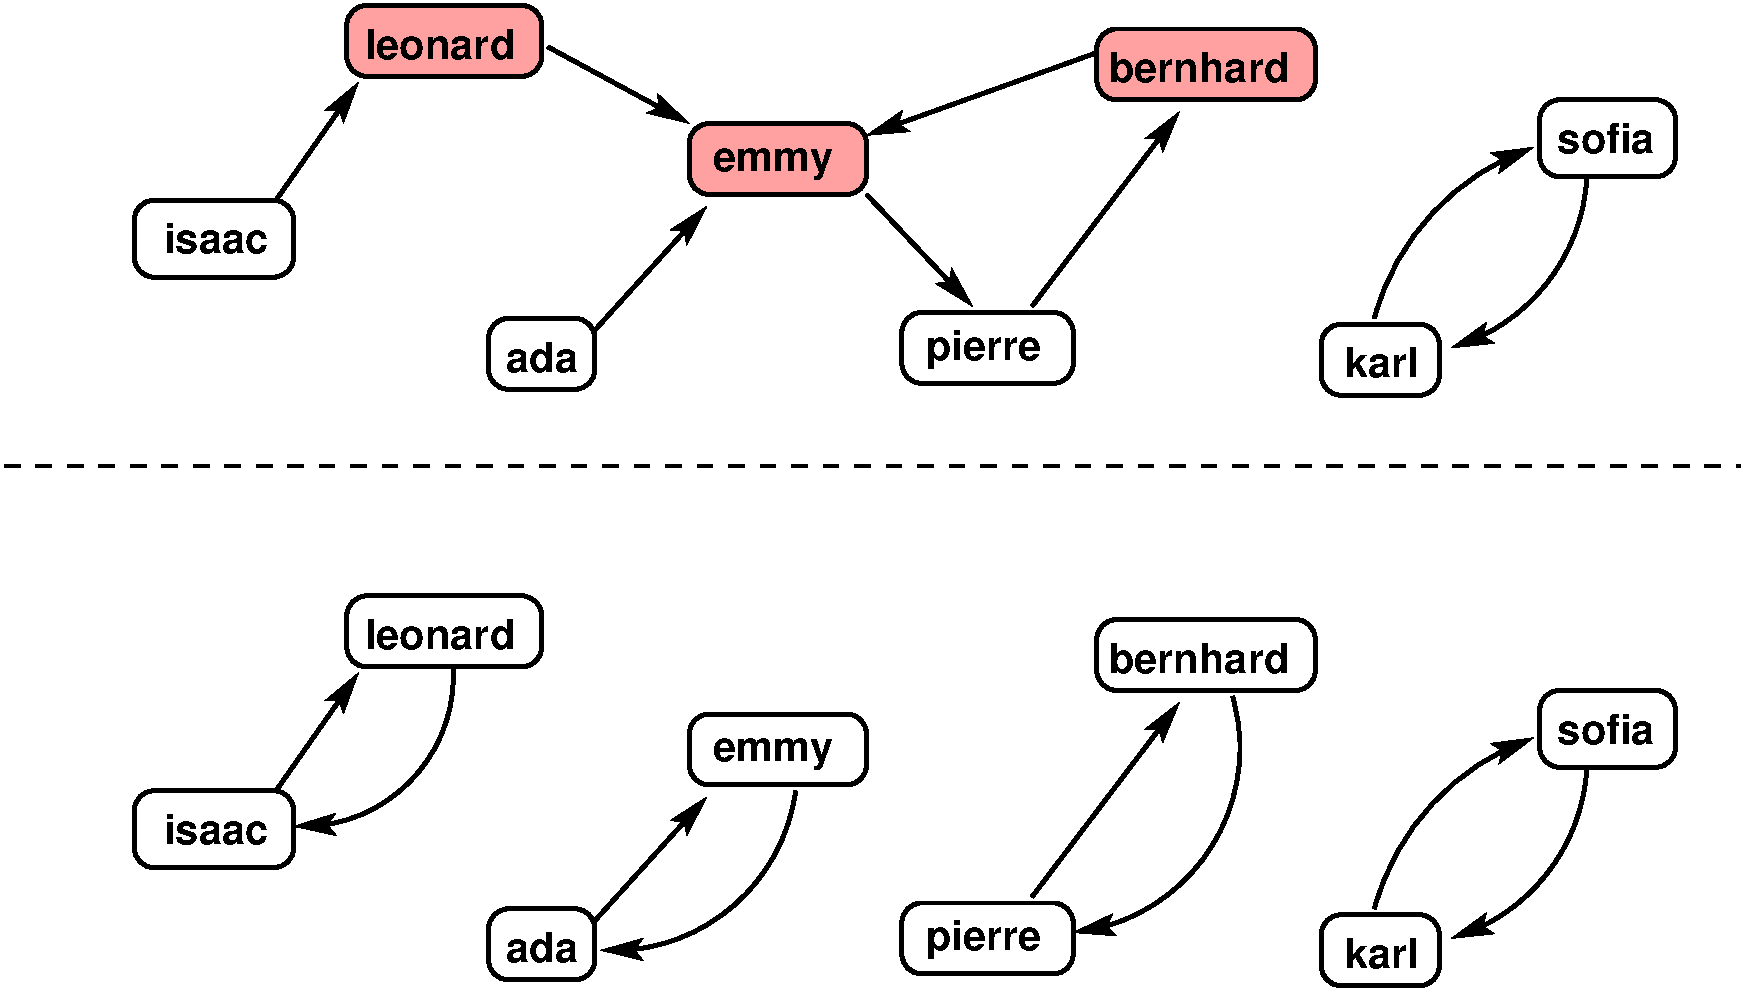
\includegraphics[width=0.5\textwidth]{polygonfig.pdf}
\end{center}

Det første eksempelet er vist i illustrasjonen over. Den øvre seksjonen viser den opprinnelige situasjonen, med en pil pekende fra $s$ til $t$ 
for å indikere at $s$ opprinnelig elsker $t$, og den rosa fargen markerer de tre karakterene som må bli skutt med
kjærlighetspiler i den unike optimale løsningen. Den nedre seksjonen viser situasjonen etterpå.

%In the first example, there is a unique optimal solution: shoot 
%which consists of shooting \texttt{b}, \texttt{d} and \texttt{f} with love arrows, having them fall in love with \texttt{h}, \texttt{c} and \texttt{e}, respectively.

I det andre eksemplet (som tilfredsstiller begrensningene i gruppe 3) så er det flere forskjellige optimale løsninger.
En av de er å skyte \texttt{a}, \texttt{b} og \texttt{d} med kjærlighetspiler, og å få de til å forelske seg i henholdsvis \texttt{b}, \texttt{a} og \texttt{c}.

I det tredje eksempelet har vi et kjærlighetstriangel, hvor uansett hvor mange piler vi skyter så vil alltid noen være utelatt.
